\documentclass[a4paper,11pt]{scrartcl}

\usepackage[ngerman]{babel} 
\usepackage[T1]{fontenc}
\usepackage[utf8]{inputenc}
\usepackage{hyperref}

\usepackage{amsmath,amsfonts,amssymb}
\usepackage{graphicx}
\usepackage{siunitx}

\usepackage{epstopdf}

\setcounter{section}{5}


\begin{document}
\hfill Alexander Schnapp

\hfill Max Menges

\hfill introhpc02

\begin{center}
\underline{\Huge{Intro HPC: Blatt 5}}\\
\large{24.11.1014}\\
\end{center}

\subsection{Heat Relaxation -- Sequential Implementation}

Der Quelltext liegt unter \verb+../5/heat.cpp+, da liegt auch ein \verb+Makefile+. Zum compilieren \verb+make+ eingeben. Das copiliert dann mit Optimierung \verb+-O2+. Zum ausführen \verb+make run n=128 it=100+ eingeben, optional zum visualisieren: \verb+make gif n=128 it=100+. Das erzeugt ein \verb+animation.gif+ im \verb+out+ Ordner.

\subsection{Heat Relaxation - Experiments}

Für die Anzahl $Flops$ gilt in Abhängigkeit von der Grid size $n$:
\begin{align*}
    Flops = 7 \cdot n^2 - 4n + 4
\end{align*}

Die Messungen wurden mit jeweils 100 Iterationen durchgeführt. Initialisierung und Output wurde nicht mitgemessen, dafür allerdings die Zeit die Benötigt wird, das Grid zu kopieren. 

Man sieht, dass die GFLOPs zunächst mit steigender Grid größe ebenfalls zunehmen, ab 512x512 aber wieder abfallen. 

Das Problem ist zunächst Computationally bound, größere Grids führen zu mehr Flops. Abeiner Grid größe von ca. 512x512 dann aber Memory bound, da die Grids nicht mehr in den Cache passen. Bei 1024x1024 ist ein double Grid $8MB$ was fast der L3-Cache größe von $10MB$ entspricht. Es müssen aber 2 Grids (für Iterationsschritte $t$ und $t+1$) im Chache gehalten werden. \\


\begin{tabular}{|c|r|r|r|}
\hline 
\multicolumn{1}{|c|}{Grid size} & \multicolumn{1}{|c|}{Time/iteration} & \multicolumn{1}{|c|}{Flops total} & \multicolumn{1}{|c|}{GFLOP/s} \\
\hline
128 x 128   &0.000106 &114,688 & 1.077\\
\hline
256 x 256   &0.000303 &458,752 & 1.512 \\
\hline
512 x 512   &0.000932 &1,835,008 & 1.968 \\
\hline
1024 x 1024 &0.004582  &7,340,032 & 1.609 \\
\hline
2048 x 2048 &0.029858 & 29,360,128&  0.983\\
\hline
4096 x 4096 &0.119876 & 117,440,512& 0.979 \\
\hline
\end{tabular} 

\begin{figure}[htbp]
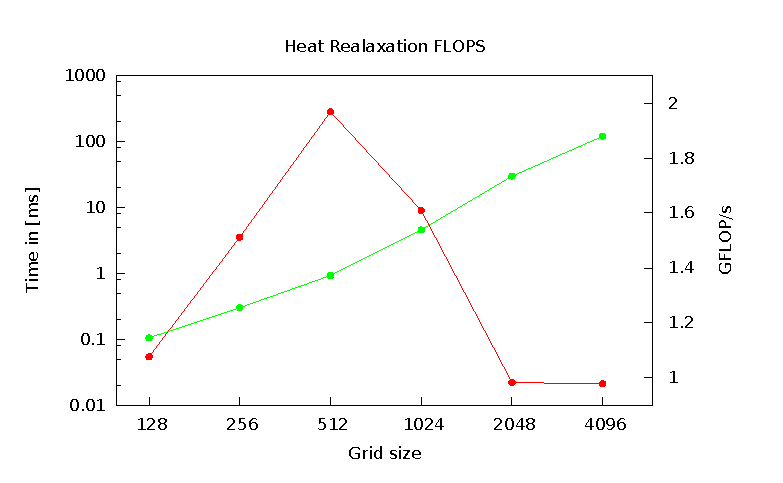
\includegraphics[width=\linewidth,
keepaspectratio]{plot.eps}
\centering
\end{figure}

\subsection{Heat Relaxation – Pre-considerations for parallelization}

In dem Falle wäre vermutlich eine 2D Zerlegung der Problems am sinnvolsten, zumindest für größere Grids.
\begin{itemize}
    \item 1D Spaltenweise 

\end{itemize}

\begin{figure}[htbp]
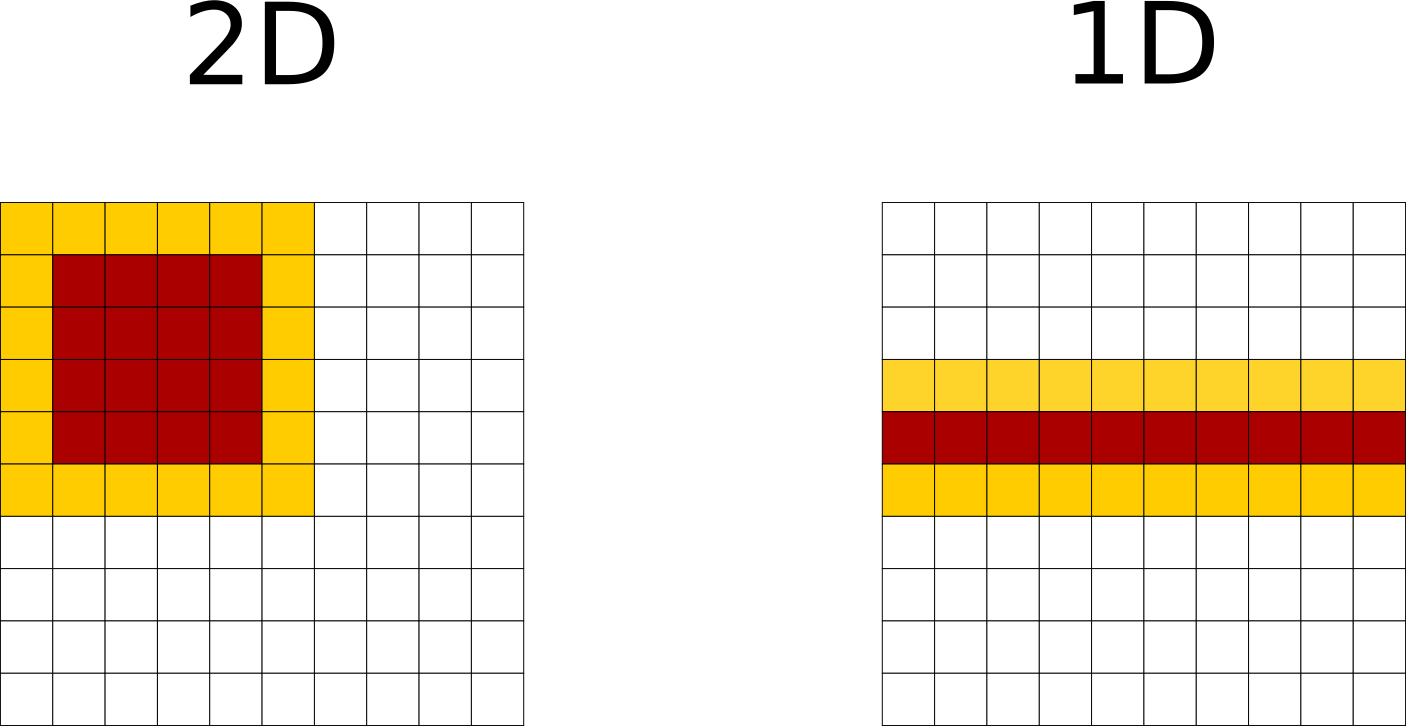
\includegraphics[width=0.7\linewidth,
keepaspectratio]{decomp.png}
\centering
\end{figure}

\end{document}
